\begin{figure*}[!t]
\centering
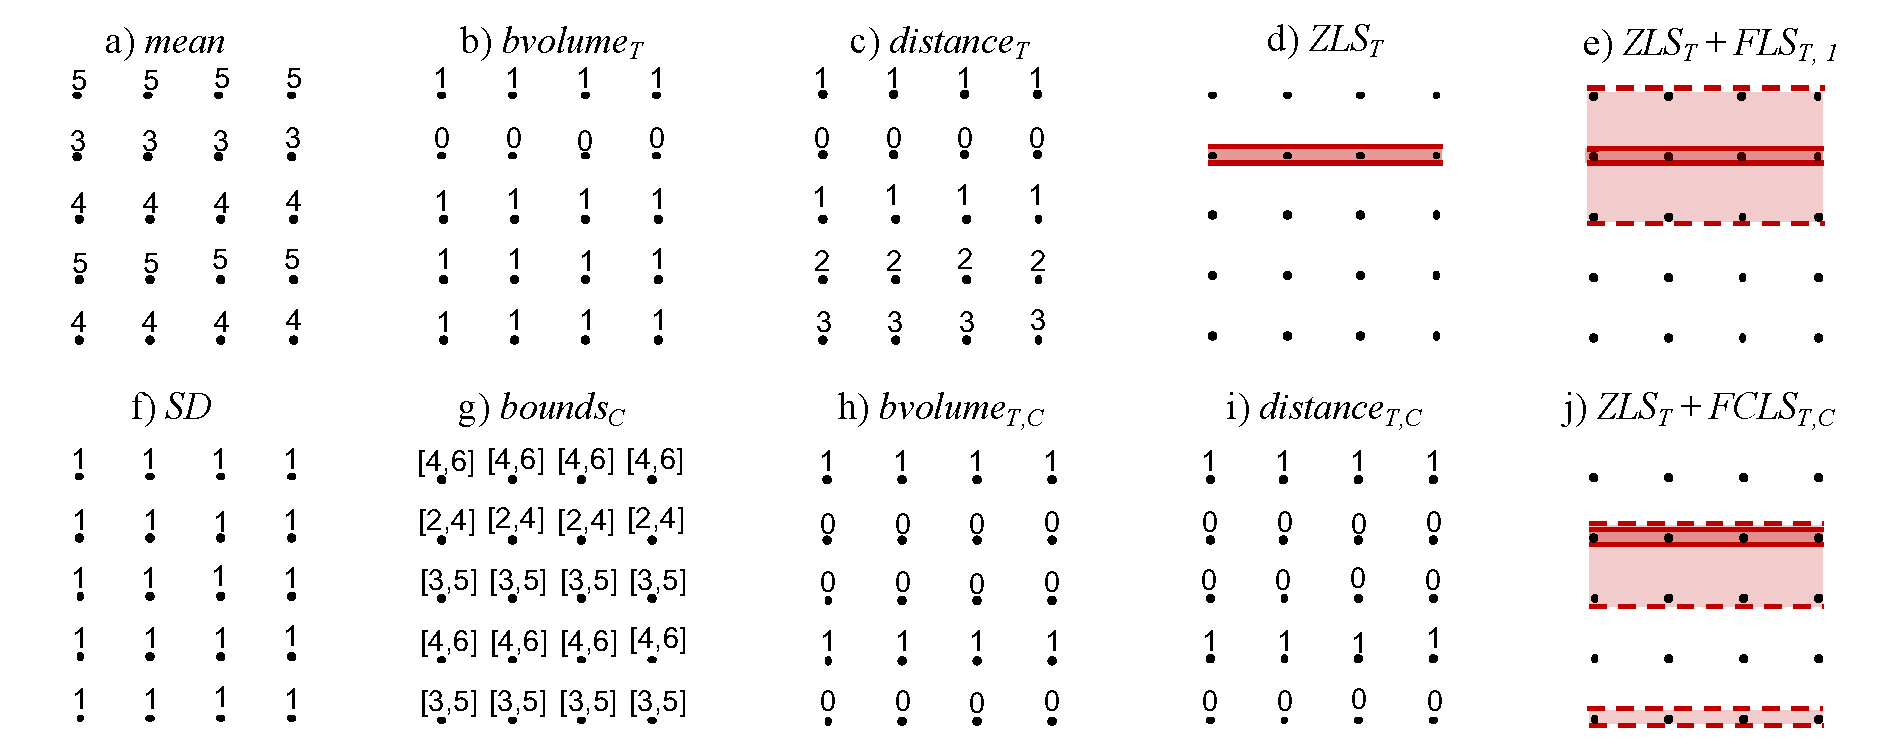
\includegraphics[width=\linewidth]{Images/example.pdf}
\vspace{-5mm}
\caption{A notional example showing the steps involved in generating feature level-sets $FLS_{T}$ and feature confidence level-set $FCLS_{T,C}$ for an uncertain univariate field represented using $mean$~(a) and $SD$~(f). For this example, we use trait $T=[2.5, 3.5]$ and confidence $C=68\%$, i.e., $Z=1$. The top row~(b-e) shows the steps to compute $FLS_{T}$. The bottom row~(g-j) shows the steps to compute $FCLS_{T}$. $ZLS_{T}$ represents the ``zero'' level-set extracted using $distance_{T}$.}
% In comparison to using $FLS_{T}$, for uncertain multivariate data, by leveraging the information pertaining to field distribution ($mean$, $SD$), $FCLS_{T,C}$ can provide a confidence controlled visualization of uncertain regions and improve secondary structure visualization for a specific trait.}
\vspace{-5mm}
\label{fig:example}
\end{figure*}
